\documentclass[12pt]{article}
\usepackage[a4paper, margin=.30in]{geometry}
\usepackage{graphicx ,
            wrapfig,
            xcolor, 
            enumerate,
            amsmath,fontenc, mhchem
            }

\newcommand\headerMe[2]{\noindent{}#1\hfill#2}
\renewcommand{\thesection}{\Roman{section}}

\author{Zakaria HAOUZAN}
\date{\today}

\begin{document}
% headers --------------
\headerMe{Matière : Physique-Chimie}{Professeur : Zakaria HAOUZAN}\\
\headerMe{Unité : Transformations lentes et rapides\\ d'un système chimique }{Établissement : Lycée SKHOR qualifiant}\\
\headerMe{Niveau : 2BAC-SM-X}{Heure : 2H}\\

% ------Content ________
\begin{center}

    \Large{Leçon $N^{\circ} 2 $: \color{red} Transformations lentes et rapides }
\end{center}

%\begin{wrapfigure}[10]{r}{0.5\textwidth}
%    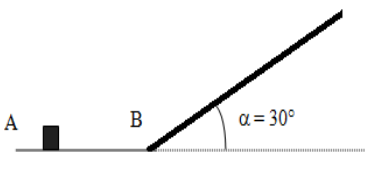
\includegraphics[width=0.5\textwidth]{./img/img00.png}
%\end{wrapfigure}


%\begin{center}
   %\begin{tabular}{|c|c|c|}
      %\hline
      %Indicateur coloré & Couleur de l’espèce acide & Couleur de l’espèce base\\\hline
      %BBT               & Jaune                     & Bleue\\\hline
      %Hélianthine       &Rose                       & Jaune\\\hline
      %Phénolphtaléine   & inclore                   & rose \\\hline
   %\end{tabular}
%\end{center}
\section*{Situation problème : Le mystère du feu d'artifice}
Lors de la fête nationale, Léa observe un magnifique feu d'artifice. Elle remarque que certaines fusées produisent des étincelles qui durent longtemps, tandis que d'autres créent des explosions de couleur rapides et intenses. Intriguée, elle se demande pourquoi il y a une telle différence dans la durée et l'intensité des réactions chimiques qui produisent ces effets lumineux.

Questions :

\begin{enumerate}
  \item  Quels types de transformations chimiques pourraient expliquer les étincelles qui durent longtemps ?
  \item  Quels facteurs pourraient influencer la vitesse des réactions dans les feux d'artifice ?
  \item  Pourquoi certaines couleurs apparaissent-elles instantanément tandis que d'autres semblent se développer plus lentement ?
\end{enumerate}


\textbf{Solutions :}

\begin{enumerate}
  \item  Les étincelles qui durent longtemps sont probablement le résultat de transformations lentes. Ces réactions pourraient impliquer la combustion contrôlée de certains métaux, comme le fer ou le titane, qui brûlent lentement dans l'air.
  \item Plusieurs facteurs peuvent influencer la vitesse des réactions dans les feux d'artifice :
  \begin{itemize}
    \item La température : les températures élevées accélèrent généralement les réactions.
    \item La taille des particules : des particules plus fines réagissent plus rapidement.
    \item La présence de catalyseurs : certains composés peuvent accélérer les réactions sans être consommés.
  \end{itemize}
\item Les couleurs qui apparaissent instantanément sont probablement le résultat de transformations rapides, comme l'excitation et la désexcitation rapide des atomes de certains métaux (par exemple, le strontium pour le rouge, le baryum pour le vert). Les couleurs qui se développent plus lentement pourraient être dues à des réactions plus complexes ou à des transformations lentes impliquant la formation progressive de composés colorés.
\end{enumerate}



\section{Introduction aux réactions d'oxydoréduction: }
Les réactions d'oxydoréduction impliquent un transfert d'électrons entre des espèces chimiques.

{Définitions importantes :} 

\begin{itemize}
  \item Oxydation : perte d'électrons.
  \item Réduction : gain d'électrons
  \item Oxydant : espèce qui gagne des électrons
  \item Réducteur : espèce qui perd des électrons
\end{itemize}

Exemple :

Considérons la réaction entre le fer et les ions cuivre (II) :
\ce{Fe + Cu^{2+} -> Fe^{2+} + Cu}

\section*{Exercice d'application 1  : }
\begin{enumerate}
	\item Écrire les demi-équations d'oxydo-réduction pour chacun des couples suivants: $Al^{3+}/Al$ ; $Cl_2/Cl^-$ ; $MnO_4^-/Mn^{2+}$ ; $Fe^{3+}/Fe^{2+}$
	\item Écrire l'équation d'oxydo-réduction entre les ions ferreux $Fe^{2+}$ et les ions permanganates $MnO_4^-$ en milieu acide sachant que  
\end{enumerate}

\begin{wrapfigure}[2]{r}{0.2\textwidth}
	\vspace{-1.95cm}
	\includegraphics[width=0.2\textwidth]{./img/TRLprecipitationChlorure.png}
\end{wrapfigure}


\section{Transformations lentes et transformations rapides : }
\subsection{Transformations rapides :  }
\subsubsection{ Définition: }
Une transformation rapide est une transformation qui se fait en une courte durée de telle façon qu'on ne peut pas suivre son
évolution en fonction du temps avec l'œil ou avec les appareils de mesure.

\subsubsection{Exemple pratique :}

\section*{Précipitation du chlorure d'argent.}
\textbf{Expérience :}

\begin{enumerate}
  \item Versez une solution de nitrate d'argent $(Ag^+ + NO_3^-)$ dans un tube à essai.
  \item Ajoutez une solution d'acide chlorhydrique $(H_3O^+  + Cl^-)$.
  \item Observez la formation immédiate d'un précipité blanc de chlorure d'argent.
  \item Équation : $\ce{Ag^+_{(aq)} +Cl^-_{(aq)} -> AgCl_{(s)} }$
  \item Application : Cette réaction est utilisée dans la photographie argentique pour créer l'image sur le film.
\end{enumerate}

\section*{Précipitation de l'hydroxyde de fer III.}
On verse dans un tube à essaies une solution de chlorure de fer III $(Cl^- +Fe^{3+} )$ puis on lui ajOute une solution d'hydroxyde de sodium $(Na^+ + OH^-)$
solution d'hydroxyde de sodium

On constate la formation d'un précipité de couleur rouille d'hydroxyde de fer III selon une réaction rapide dont l'équation s'écrit: \ce{Fe^{3+}_{(aq)}  + 3HO^-_{(aq)} -> Fe(OH)_3}

\begin{figure}[h!]
	\begin{center}
	\includegraphics[width=0.4\textwidth]{./img/TRLtestchimique.png}

	\includegraphics[width=0.4\textwidth]{./img/TRLidurelente.png}
\end{center}
\vspace{-1cm}
\end{figure}

\subsection{Transformations lentes :}
\subsubsection{Définition: }
Une transformation lente est une transformation qui se fait dans une certaine durée de telle façon qu'on suivre son évolution en
fonction du temps avec l'œil ou avec les appareils de mesure.

\section*{Exemple pratique :  }
Réaction entre les ions iodure $(I^-)$ et l'eau oxygénée $(H_2O_2)$ (peroxyde d'hydrogéne)

\begin{itemize}
  \item On verse dans un tube à essaies une solution d'iodure de potassium $(K^+ + I^-)$ puis on lui ajoute un peu d'eau oxygénée $(H_2O_2)$ acidifiée (avec quelques gouttes d'acide sulfurique $H_2SO_4$)
  \item On constate que la couleur du mélange réactionnel
évolue progressivement du jaune au jaune foncé puis prend une coloration brune qui devient de plus en plus foncée en fonction du
temps .
\item Donc la réaction des ions iodures $I^-$ et les molécules $H_2O_2$ est une réaction lente au cours de laquelle les
	ions iodures s'oxydent selon la demi-équation suivante: 

	\ce{2I^- <=> I_2 + 2e^-}
\item Alors que les molécules H2O2 se réduisent selon la demi-équation suivante: 

	\ce{H_2O_2 + 2H^+ + 2e^- <=> 2H_2O}

\item L'équation bilan d'oxydo-réduction: \ce{H_2O_2 + 2I^- + 2H^+ ->[\text{réaction lente}] I_2 + 2H_2O}

\item Application : Cette réaction est utilisée dans certains tests de détection de peroxyde d'hydrogène.
\end{itemize}
\section{Les facteurs cinétiques }
\subsection{Définition: }
On appelle facteur cinétique tout paramètre capable d'influer sur la vitesse d'une transformation chimique.

\subsection{Influence des facteur cinétique sur la vitesse de la réaction:}
\subsubsection{Influence de la température: }

Règle générale : Une augmentation de la température accélère la réaction.

D'une manière générale, plus la température du milieu réactionnel est élevée, plus la transformation est rapide. Inversement plus la température du milieu est basse plus la transformation est lente.

Applications:	On accélère certaines transformations dans l'industrie pour les rendre plus rentables.

On refroidit brutalement certains milieux réactionnels pour "arrêter" certaines transformations (on réalise ainsi ce qu'on appelle une "trempe").

Un réfrigérateur et un congélateur permettent de ralentir les transformations de dégradation biochimiques des aliments.

Dans l'exemple ci-dessous, les ions permanganate $MnO_4^-$ en milieu acide réagissent avec l'acide oxalique 
 (éthanedioïque) $H_2C_2O_4$. Dans le bécher de droite le mélange est plongé dans un bain Marie à 40°C. Dans le bécher de gauche le mélange est plongé dans un bain Marie à 20°C.
\begin{figure}[h!]
	\begin{center}
	\includegraphics[width=0.5\textwidth]{./img/TRLtemperatureFact.png}
\end{center}
\vspace{-1cm}
\end{figure}

\subsubsection{Influence de la concentration initiale des réactifs :}
Règle générale : Des concentrations plus élevées accélèrent la réaction.

D'une manière générale, plus les concentrations initiales des réactifs sont élevées plus la transformation est rapide.

Dans l'exemple ci-dessous, la réaction entre les ions thiosulfate et les ions oxonium produit du soufre en suspension qui rend la solution opaque. A droite la concentration initiale en ions thiosulfate est deux fois plus élevée qu'à gauche.
\begin{figure}[h!]
	\begin{center}
	\includegraphics[width=0.5\textwidth]{./img/TRLconcentration.png}
\end{center}
\vspace{-1cm}
\end{figure}

On constate que la vitesse de la réaction est d'autant plus grande que la concentration initiale de l'un des réactif est plus grande.
Donc la concentration initiale des réactifs est un facteur cinétique.

\textbf{Remarque : Il existe d'autres facteurs cinétiques comme le catalyseur et la nature du solvant}

\section{Quelques application des facteurs cinétiques}
\begin{itemize}
	\item On peut ralentir ou accélérer une transformation chimique en agissant sur les facteurs cinétiques.
	\item On accélère des transformations en augmentant la température du milieu réactionnel.
	\item On ralentit ou on bloque des transformations, on contrôle des réactions dangereuses, on diminuant la température ou en diluant le mélange réactionnel.
\end{itemize}



\end{document}

